% Preamble
% --------
\documentclass[12pt]{article}

% Packages
% --------
\usepackage{blindtext} %for boilerplate text (\blindtext)
\usepackage{geometry} %for paper dimensions and margins
\usepackage{graphicx} % for including graphics

% Page Setup
% ----------
\geometry{letterpaper, margin=1in}

% Title content and formatting
% ----------------------------
\title{Apex Instruction Set Architecture Simulator (\texttt{apex-sim}) \\ Phase 1 Documentation}
\author{Matthew Cole \\ \texttt{mcole8@binghamton.edu}
\and
Brian Gracin \\ 
	\texttt{bgracin1@binghamton.edu}}
\date{19 November 2016} % or to emit: \date{\today}

\begin{document}
% Emit title content
% ------------------
\pagenumbering{gobble}
\maketitle
\tableofcontents
\listoffigures
\newpage
\pagenumbering{arabic}

\section{Design}
\blindtext

\subsection{Driver Program}

\subsection{Classes}

\begin{figure}
  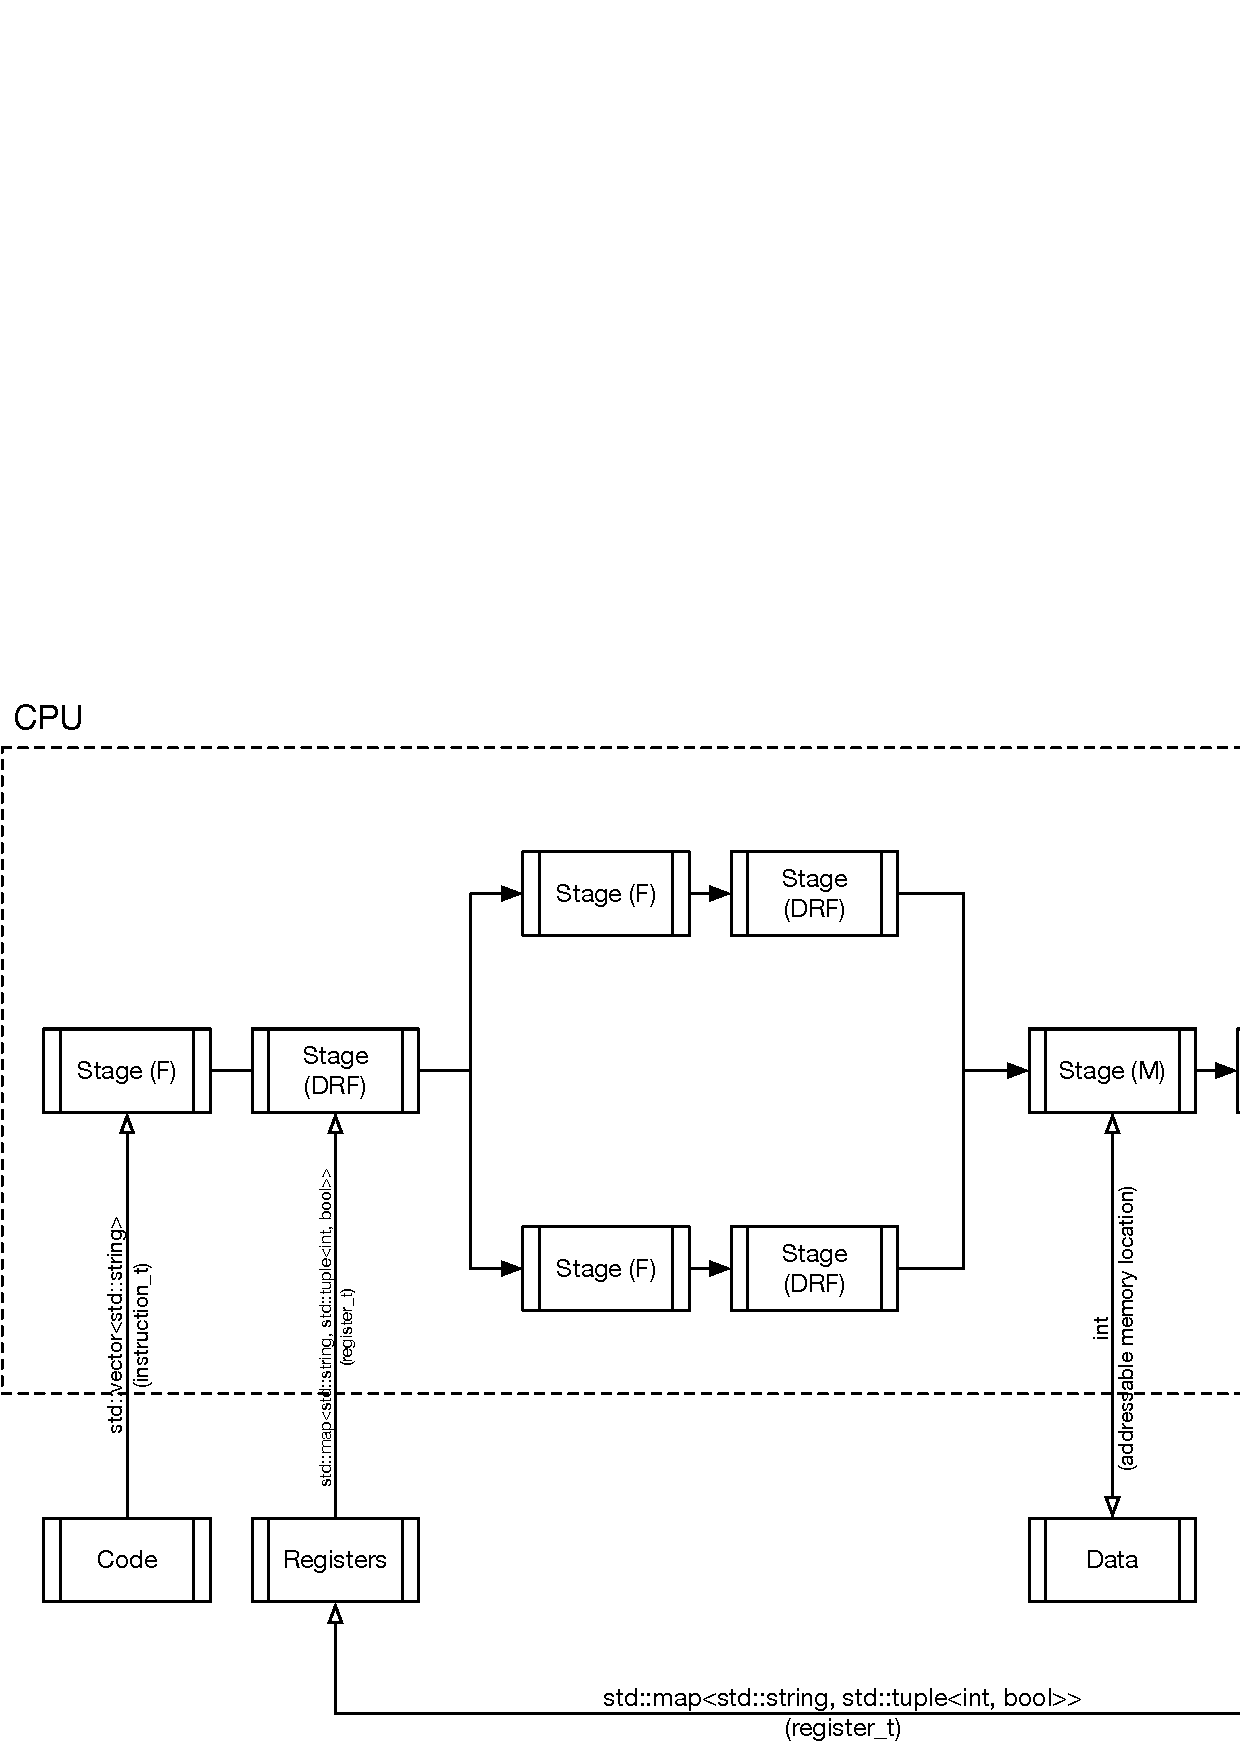
\includegraphics[width=\linewidth]{./figs/apex-sim-overview.pdf}
  \caption{The APEX pipeline and class interactions.}
  \label{fig:overview}
\end{figure}

Figure \ref{fig:overview} shows class interactions and data flow between each of the stages and support classes.

\subsubsection{Code}

\subsubsection{Data}

\subsubsection{Registers}

\subsubsection{CPU}

\section{Implementation}
\subsection{Stages}

\subsection{Stalls}

\subsection{Forwarding}

\section{Work Log}
\blindtext

\end{document}


